
%(BEGIN_QUESTION)
% Copyright 2006, Tony R. Kuphaldt, released under the Creative Commons Attribution License (v 1.0)
% This means you may do almost anything with this work of mine, so long as you give me proper credit

Øker eller \textit{minker} utgangstrykket fra dette reléet når inngangstrykket øker?  Med andre ord: er dette et \textit{direktevirkende} eller \textit{reversvirkende} relé?

$$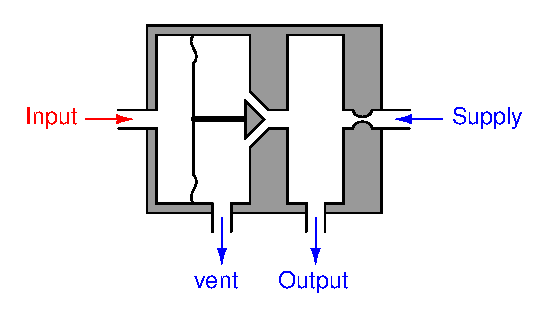
\includegraphics[width=15.5cm]{i00197x01.eps}$$

\vskip 20pt \vbox{\hrule \hbox{\strut \vrule{} {\bf Suggestions for Socratic discussion} \vrule} \hrule}

\begin{itemize}
\item{} Forklar sammenligningen: ``Et relé er for en pilotventil det en transistor er for en håndbryter''
\item{} Hvordan tror du lekkasje eller rift i membranen vil påvirke oppførselen til dette reléet?
\item{} Hvordan tror du en tett orifice vil påvirke oppførselen til dette reléet?
\item{} Hvordan tror du variasjoner i forsyningstrykket vil påvirke oppførselen til dette reléet?
\end{itemize}

\underbar{file i00197}
%(END_QUESTION)





%(BEGIN_ANSWER)


%(END_ANSWER)





%(BEGIN_NOTES)

Utgangstrykket øker når inngangstrykket øker: dette er et \textit{direktevirkende} relé.






\vfil \eject

\noindent
{\bf Summary Quiz:}

Identifiser en tilstand i dette pneumatiske reléet som vil få utgangstrykket til å synke:

$$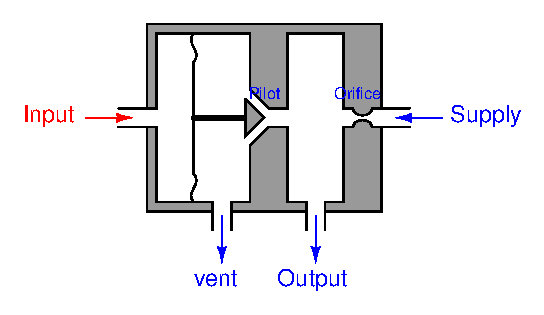
\includegraphics[width=15.5cm]{i00197x02.eps}$$

\begin{itemize}
\item{} Inngangstrykket øker
\vskip 5pt 
\item{} Smuss tetter pilotventilen
\vskip 5pt 
\item{} Smuss tetter ventilasjonshullet
\vskip 5pt 
\item{} Forsyningstrykket øker
\vskip 5pt 
\item{} Lufttemperaturen øker
\vskip 5pt 
\item{} Smuss tetter orifice
\vskip 5pt 
\item{} Lufttemperaturen synker
\end{itemize}


%INDEX% Basics, pneumatics: relay action (direct vs. reverse)

%(END_NOTES)

